% \documentclass[AMA,Times1COL]{WileyNJDv5}
\documentclass[HARVARD,LATO2COL]{WileyNJDv5}


\articletype{Article Type}%

\received{Date Month Year}
\revised{Date Month Year}
\accepted{Date Month Year}
\journal{Journal}
\volume{00}
\copyyear{2023}
\startpage{1}

\raggedbottom
\usepackage{graphicx}
\usepackage{tikz}
\usetikzlibrary{positioning,arrows.meta}
\usepackage{booktabs}
\usepackage{multirow}
\usepackage{listings}
\usepackage{url,overcite}
\usepackage{xcolor}


\begin{document}

\title{AN AIOT-Based Alcohol Level Detection and Vehicle Ignition Prevention System}

\author[1]{Anastasiia Igorevna Shaposhnikova}

\author[1]{Sudhanshu Tripathi}

\author[1]{Ram Naresh}
\author[2]{Pramod Kumar Soni}

\authormark{TAYLOR \textsc{et al.}}
\titlemark{PLEASE INSERT YOUR ARTICLE TITLE HERE}

\address[1]{\orgdiv{Department of Information Technology}, \orgname{Amity University Tashkent}, \orgaddress{\state{Tashkent}, \country{Uzbekistan}}}
\address[2]{\orgdiv{Department of Computer Applications}, \orgname{Manipal University Jaipur, Jaipur}, \orgaddress{\state{Rajasthan}, \country{India}}}
\corres{Pramod Kumar Soni \email{pramod.soni@jaipur.manipal.edu}}

\presentaddress{This is sample for present address text this is sample for present address text.}

%\fundingInfo{Text}
%\JELinfo{ejlje}

\abstract[Abstract]{This paper introduces an Alcowatch system that utilizes wearable technology to estimate blood alcohol concentration (BAC) and includes a fail-safe mechanism for vehicle ignition control. The system combines PPG, EDA, and temperature signals on a Wear OS smartwatch, uses a BiLSTM-attention model to make decisions on the device, and sends a 20-byte BAC status packet to an Arduino-based vehicle controller via BLE. A safety-aware loss function punishes false negatives, and a climate-adaptive calibration fixes for changes in temperature and humidity. The prototype was tested on synthetic physiological sequences and a hardware-in-the-loop simulator. The results showed an MAE of 0.0082 g/dL, a false negative rate of 0.7\%, an end-to-end latency of 580 ms, and a TensorFlow Lite model of 22 KB. The finite state machine on the vehicle side stops the ignition by default and makes sure that timeouts and watch-wear checks are done. }

\keywords{blood alcohol concentration, wearable sensing vehicle safety, Bluetooth Low Energy}

\jnlcitation{\cname{%
\author{Taylor M.},
\author{Lauritzen P},
\author{Erath C}, and
\author{Mittal R}}.
\ctitle{On simplifying ‘incremental remap’-based transport schemes.} \cjournal{\it J Comput Phys.} \cvol{2021;00(00):1--18}.}


\maketitle

\renewcommand\thefootnote{}
\footnotetext{\textbf{Abbreviations:} ANA, anti-nuclear antibodies; APC, antigen-presenting cells; IRF, interferon regulatory factor.}

\renewcommand\thefootnote{\fnsymbol{footnote}}
\setcounter{footnote}{1}

\section{Introducion}\label{sec1}
Driving while drunk is still a major cause of car accidents, deaths, and serious injuries around the world. Although there have been many attempts to establish laws and set up rules, it is still hard to enforce blood alcohol concentration (BAC) limits in real time \citep{lombardo2020l}. Enforcement based on traditional breathalysers is hit-or-miss, depends on the operator, and can be avoided \citep{das2023}. The need for intelligent, autonomous alcohol detection systems has led to research into wearable biosensing technologies integrated with automotive safety systems. Existing alcohol detection systems lack sophisticated software algorithms that can:  accurately estimate BAC from multimodal physiological sensor data in real-time; adapt to varying environmental conditions through intelligent calibration, ensure security against spoofing and tampering through software-based authentication, and  provide longitudinal behavioural tracking capabilities. There is a need for advanced system that address these challenges while maintaining computational efficiency suitable for resource-constrained wearable devices. \par
Current alcohol detection systems primarily rely on breathalyzer mechanisms or in-vehicle sensors. U.S. Patents 5,736,965 and 7,113,834 describe vehicle ignition lockout mechanisms based on breath alcohol content \citep{uspat5736965, uspat7113834}. Indian Patent No. 286703 integrates breath analyzers with GSM modules for remote monitoring \citep{inpat286703}. These systems, while effective, require active user participation and are vulnerable to circumvention. Fairbairn and Kang provide comprehensive insights into transdermal alcohol monitoring technologies and their software processing requirements \citep{fairbairn2021}. Recent advances in smartwatch-based prediction using hyperdimensional computing  demonstrate the feasibility of wearable devices for continuous alcohol monitoring, highlighting the importance of sophisticated signal processing algorithms \citep{verges2024}.Machine learning approaches for BAC estimation from physiological signals have shown promise in recent research. Sensor fusion techniques combining multiple physiological parameters improve accuracy compared to single-sensor approaches and the security of the system also remain major concern to prevent unauthorized access and manipulation \citep{sensors2024, sensors2023}.


However, challenges remain in developing algorithms that generalize across diverse populations and environmental conditions while maintaining computational efficiency for embedded deployment. The AlcoWatch EMA framework represents an innovative software approach for high-temporal-density, longitudinal measurement of alcohol use \citep{alcowatch2025}. This software architecture enables behavioural tracking and intervention capabilities that extend beyond simple detection to comprehensive alcohol use profiling and analysis.
\par
\begin{figure*}[t]
\centering
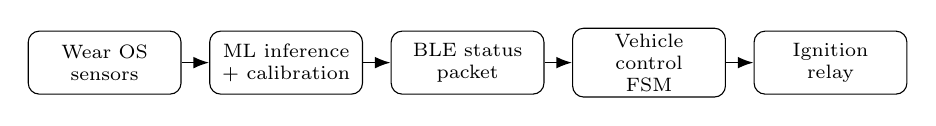
\begin{tikzpicture}[node distance=0.35cm, >=Latex, font=\scriptsize]
\tikzstyle{block} = [draw, rounded corners, align=center, text width=1.8cm, minimum height=0.8cm, inner sep=2pt]
\tikzstyle{link} = [->, line width=0.6pt]

\node[block] (watch) {Wear OS\\sensors};
\node[block, right=of watch] (ml) {ML inference\\+ calibration};
\node[block, right=of ml] (ble) {BLE status\\packet};
\node[block, right=of ble] (vehicle) {Vehicle control\\FSM};
\node[block, right=of vehicle] (relay) {Ignition\\relay};

\draw[link] (watch) -- (ml);
\draw[link] (ml) -- (ble);
\draw[link] (ble) -- (vehicle);
\draw[link] (vehicle) -- (relay);
\end{tikzpicture}

\caption{Architecture and data flow of the proposed system.}
\label{fig:system}
\end{figure*}

\begin{figure*}[t]
\centering
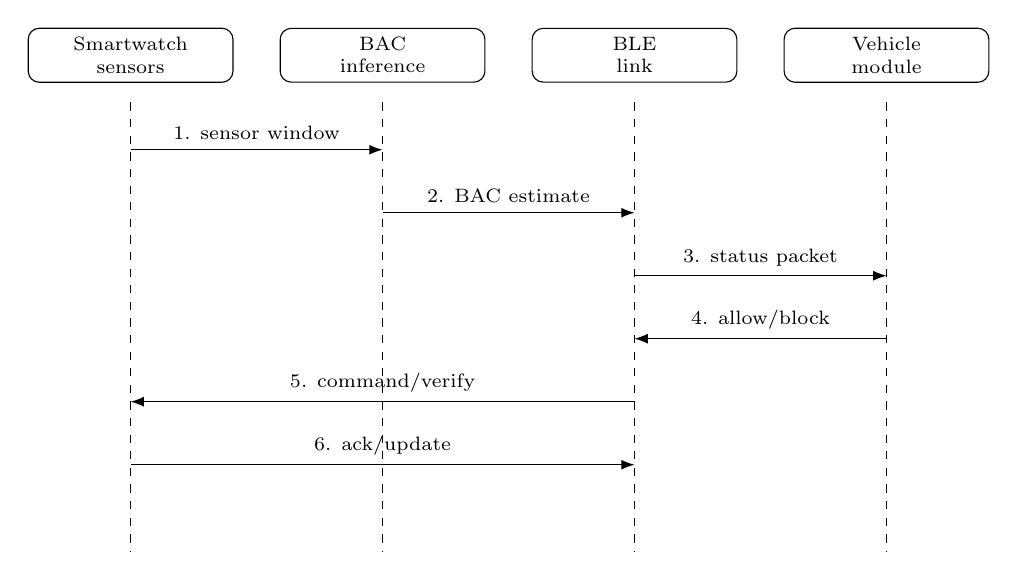
\begin{tikzpicture}[x=1cm,y=1cm,font=\scriptsize,>=Latex]
\node[draw, rounded corners, align=center, minimum width=2.6cm] (sw) at (1.3,0) {Smartwatch\\sensors};
\node[draw, rounded corners, align=center, minimum width=2.6cm] (ml) at (4.5,0) {BAC\\inference};
\node[draw, rounded corners, align=center, minimum width=2.6cm] (ble) at (7.7,0) {BLE\\link};
\node[draw, rounded corners, align=center, minimum width=2.6cm] (veh) at (10.9,0) {Vehicle\\module};

\draw[dashed] (1.3,-0.6) -- (1.3,-6.3);
\draw[dashed] (4.5,-0.6) -- (4.5,-6.3);
\draw[dashed] (7.7,-0.6) -- (7.7,-6.3);
\draw[dashed] (10.9,-0.6) -- (10.9,-6.3);

\draw[->] (1.3,-1.2) -- (4.5,-1.2) node[midway, above]{1. sensor window};
\draw[->] (4.5,-2.0) -- (7.7,-2.0) node[midway, above]{2. BAC estimate};
\draw[->] (7.7,-2.8) -- (10.9,-2.8) node[midway, above]{3. status packet};
\draw[->] (10.9,-3.6) -- (7.7,-3.6) node[midway, above]{4. allow/block};
\draw[->] (7.7,-4.4) -- (1.3,-4.4) node[midway, above]{5. command/verify};
\draw[->] (1.3,-5.2) -- (7.7,-5.2) node[midway, above]{6. ack/update};
\end{tikzpicture}

\caption{Operational sequence from sensing to ignition control.}
\label{fig:sequence}
\end{figure*}

In this work an alcohol detection system is designed using wearable sensors, vehicle control modules, and communication devices that that processes sensor data, estimates BAC levels, makes ignition control decisions, and ensures secure data transmission. This work demonstrates how the proposed system can bridge wearable biosensing technology with automotive control systems to create an intelligent safety mechanism. The main contribution of this work are as follows:
\begin{enumerate}
    \item Design and implement AI/ML algorithms for real-time BAC estimation from multimodal sensor data
    \item Develop sensor fusion algorithms that combine PPG, EDA, and temperature data
    \item Create climate-adaptive calibration algorithms for environmental compensation
    \item Implement secure BLE communication protocols with AES-256 encryption
    \item Design ignition control decision-making logic and state machine
    \item Develop biometric authentication algorithms for continuous user verification
    \item Create the AlcoWatch EMA framework for longitudinal tracking
    \item Optimize software for resource-constrained embedded environments
\end{enumerate}

\section{Methodology}\label{sec2}
The AlcoWatch system implements a distributed software architecture across three computing platforms: (1) a Wearable OS smartwatch application for sensor data acquisition and BAC estimation, (2) an Arduino-based vehicle control module for ignition management, and (3) BLE communication middleware for secure data exchange. Figure~\ref{fig:system} illustrates the complete system architecture and data flow.
The system follows a distributed computing model where processing is split between the wearable device and vehicle module to optimize for power efficiency and real-time performance. The smartwatch runs computationally intensive machine learning inference, while the Arduino implements safety-critical decision logic with fail-safe guarantees. Figure~\ref{fig:sequence} summarizes the operational sequence from sensing to ignition control. The complete data flow of this sequence is as follows:
\begin{enumerate}
    \item Physiological sensors (PPG, EDA, temperature) capture raw signals at 64 Hz
    \item Signal processing algorithms extract features and remove noise
    \item TensorFlow Lite model performs BAC inference on 10-timestep sequences
    \item Climate-adaptive calibration adjusts estimates for environmental conditions
    \item BLE peripheral broadcasts 20-byte status packets every 30 seconds
    \item Arduino BLE central receives and validates packet integrity
    \item Ignition control state machine makes enable/disable decisions
    \item Visual and audio feedback provides driver notifications
\end{enumerate}
\subsection{Neural Network Architecture}
The BAC estimation model employs a specialized temporal sequence processing architecture combining Bidirectional Long Short-Term Memory (BiLSTM) networks with an attention mechanism. Table~\ref{tab:model_arch} provides the complete network specification.
\begin{table}[htbp]
\caption{Neural Network Architecture Specifications}
\label{tab:model_arch}
\centering
\small
\begin{tabular}{@{}lll@{}}
\toprule
\textbf{Layer} & \textbf{Configuration} & \textbf{Output Shape} \\
\midrule
Input & 10 timesteps $\times$ 6 features & [batch, 10, 6] \\
BiLSTM & 64 units, return sequences & [batch, 10, 128] \\
Dropout & Rate = 0.3 & [batch, 10, 128] \\
Attention & Temporal attention weights & [batch, 128] \\
Dense & 32 units, ReLU & [batch, 32] \\
Dropout & Rate = 0.3 & [batch, 32] \\
Dense & 16 units, ReLU & [batch, 16] \\
Output & 1 unit, Linear & [batch, 1] \\
\bottomrule
\end{tabular}
\end{table}
The input layer accepts sequences of 10 time steps (representing 5 minutes of measurements at 30-second intervals) with 6 physiological features per time step. The BiLSTM layer processes sequences in both forward and backward temporal directions, enabling the model to capture both past and future context for each timestep. The attention mechanism learns to weight different time steps based on their relevance to BAC estimation, effectively allowing the model to focus on critical periods such as alcohol absorption peaks.
\subsection{Feature Extraction}
Table~\ref{tab:features} describes the six physiological features used for BAC estimation. These features were selected based on their physiological correlation with alcohol consumption and availability on commercial Wear OS devices. Feature normalization is performed using pre-computed mean and standard deviation values derived from the training dataset: \begin{equation}
x_{norm} = \frac{x - \mu}{\sigma}
\end{equation}

where $\mu$ and $\sigma$ are the feature-specific normalization parameters stored in the model metadata. 

\begin{table}[htbp]
\caption{Input Features for BAC Estimation}
\label{tab:features}
\centering
\small
\begin{tabular}{@{}llll@{}}
\toprule
\textbf{Feature} & \textbf{Range} & \textbf{Unit} & \textbf{Correlation} \\
\midrule
PPG Heart Rate & 60-150 & bpm & $+$0.82 \\
PPG Quality & 0.5-1.0 & - & $-$0.68 \\
EDA Value & 2-20 & $\mu$S & $+$0.75 \\
Skin Temperature & 32-34 & $^\circ$C & $+$0.71 \\
Ambient Temp. & 20-30 & $^\circ$C & Calibration \\
Humidity & 30-70 & \% & Calibration \\
\bottomrule
\end{tabular}
\end{table}
\subsection{Custom Loss Function for Safety}
A critical part of the model design is the safety-aware loss function that asymmetrically penalizes prediction errors. False negatives (predicting low BAC when actual BAC is high) are significantly more dangerous than false positives in a safety-critical system. The custom loss function is defined as:

\begin{equation}
\mathcal{L} = \text{MSE}(y, \hat{y}) + 5 \cdot \sum_{i} \mathbb{1}_{y_i > \tau \land \hat{y}_i < \tau} (y_i - \hat{y}_i)^2
\end{equation}

where $y$ is the true BAC, $\hat{y}$ is the predicted BAC, $\tau = 0.08$ g/dL is the legal threshold, and $\mathbb{1}$ is the indicator function. This formulation applies a 5$\times$ penalty multiplier to false negative cases, encouraging the model to err on the side of caution.
\subsection{Climate-Adaptive Calibration Algorithm}
The climate-adaptive calibration algorithm that adjusts BAC predictions based on environmental conditions. Ambient temperature and humidity affect transdermal alcohol measurement accuracy through changes in skin conductivity and perspiration rates. The calibration algorithm implements region-specific correction factors as shown in Table~\ref{tab:climate}.
\begin{table}[htbp]
\caption{Climate-Adaptive Calibration Parameters}
\label{tab:climate}
\centering
\small
\begin{tabular}{@{}llll@{}}
\toprule
\textbf{Region} & \textbf{Temp Coeff.} & \textbf{Humidity Coeff.} & \textbf{Base Temp} \\
\midrule
Central Asia & 0.012 & 0.008 & 30.0$^\circ$C \\
Europe & 0.010 & 0.006 & 20.0$^\circ$C \\
Default & 0.011 & 0.007 & 25.0$^\circ$C \\
\bottomrule
\end{tabular}
\end{table}

The calibration formula applies linear adjustments based on deviation from baseline conditions:

\begin{equation}
\begin{split}
\text{BAC}_{\text{cal}} = \text{BAC}_{\text{raw}} &+ \alpha_T (T_{\text{amb}} - T_{\text{base}}) \\
&+ \alpha_H \frac{(H - 50)}{100}
\end{split}
\end{equation}

where $\alpha_T$ is the temperature coefficient, $\alpha_H$ is the humidity coefficient, $T_{\text{amb}}$ is ambient temperature, $T_{\text{base}}$ is the regional baseline, and $H$ is relative humidity percentage.

\subsection{Quantization of the Model}
To enable real-time inference on resource-constrained Wear OS devices, the trained Keras model undergoes conversion to TensorFlow Lite format with post-training quantization. Table~\ref{tab:tflite} summarizes the optimization results.

\begin{table}[htbp]
\caption{TFLite Model Optimization Results}
\label{tab:tflite}
\centering
\small
\begin{tabular}{@{}lll@{}}
\toprule
\textbf{Metric} & \textbf{Keras Model} & \textbf{TFLite Model} \\
\midrule
File Size & 1.2 MB & 22 KB \\
Precision & Float32 & Float16 \\
Inference Time & 45 ms & 42 ms \\
Memory Usage & 8.5 MB & 2.3 MB \\
MAE (g/dL) & 0.0079 & 0.0082 \\
\bottomrule
\end{tabular}
\end{table}
The quantization process reduces model size by 98.2\% while maintaining prediction accuracy within acceptable bounds. The slight increase in MAE (0.0003 g/dL) is negligible compared to the substantial resource savings. Dynamic range quantization is employed, converting weights from 32-bit to 16-bit floating-point representation while maintaining activation precision.
\subsection{Hyperparameters for Training}
Table~\ref{tab:training} provides the complete training configuration used to achieve optimal model performance. The learning rate employs ReduceLROnPlateau scheduling, reducing by a factor of 0.5 when validation loss plateaus for 5 consecutive epochs, with a minimum learning rate of $10^{-6}$.

\begin{table}[htbp]
\caption{Model Training Hyperparameters}
\label{tab:training}
\centering
\small
\begin{tabular}{@{}ll@{}}
\toprule
\textbf{Hyperparameter} & \textbf{Value} \\
\midrule
Optimizer & Adam \\
Learning Rate & 0.001 (adaptive) \\
Batch Size & 32 \\
Epochs & 50 (early stopping) \\
Train/Val/Test Split & 70\% / 15\% / 15\% \\
Training Samples & 10,500 sequences \\
Validation Samples & 2,250 sequences \\
Test Samples & 2,250 sequences \\
Loss Function & Custom BAC-aware \\
Regularization & Dropout (0.3) \\
Early Stopping Patience & 10 epochs \\
\bottomrule
\end{tabular}
\end{table}
\lstset{
  basicstyle=\ttfamily\small,
  numbers=left,
  numberstyle=\tiny,
  stepnumber=1,
  frame=single,
  rulecolor=\color{black},
  captionpos=b,
  breaklines=true,
  tabsize=2
}


\section{Experimental Results and Discussion}
In this section the hardware details used for the design of the system and the experimental results are discussed. 

\subsection{Implementation Details}

\subsubsection{Sensor Data Collection}
The application utilizes the Android Health Services API for physiological sensor access. Unlike the deprecated SensorManager API, Health Services provides optimized access to wearable sensors with improved battery efficiency and data quality. PPG data is collected at 64 Hz using the \texttt{HEART\_RATE\_BPM} data type. Since most Wear OS devices lack dedicated EDA sensors, electrodermal activity is estimated from heart rate variability (HRV) using a 10-sample rolling window:

\begin{equation}
\text{EDA}_{\text{est}} = 3.0 + \frac{\sigma_{HR}}{5.0}
\end{equation}

where $\sigma_{HR}$ is the standard deviation of heart rate over the window. 
The primary sensor data structure is defined as:
\begin{lstlisting}[language=Java, caption={Combined Sensor Data Structure (Kotlin)}, label={lst:sensordata}]
data class CombinedSensorData(
    val timestamp: Long,
    val ppgValue: Double,      // Heart rate (bpm)
    val ppgQuality: Double,    // Quality 0-1
    val edaValue: Double,      // EDA (microsiemens)
    val temperature: Double,   // Skin temp (C)
    val ambientTemp: Double,   // Ambient temp (C)
    val humidity: Double       // Relative humidity (%)
)
\end{lstlisting}
\subsubsection{Real-Time BAC Inference}
The BACInferenceEngine module implements on-device machine learning inference using the TensorFlow Lite interpreter. A circular buffer maintains the most recent 10 sensor readings for sequence-based prediction. The alert level classification follows this threshold scheme:
\begin{itemize}
    \item SAFE: BAC $< 0.05$ g/dL
    \item WARNING: $0.05 \leq$ BAC $< 0.08$ g/dL
    \item DANGER: $0.08 \leq$ BAC $< 0.15$ g/dL
    \item CRITICAL: BAC $\geq 0.15$ g/dL
\end{itemize}

Confidence scoring ranges from 0.75 to 0.95 based on sensor quality metrics and BAC value stability over recent predictions.
\subsubsection{Design and Implementation}
The AlcoWatch BLE protocol implements a custom GATT (Generic Attribute Profile) service with three characteristics for bidirectional communication namely, AlcoWatch Service, BAC Status, Vehicle Command. and System Status.
The BAC Status characteristic transmits 20-byte packets containing sensor data, BAC estimates, and system state information. Table~\ref{tab:bac_packet} details the packet structure.

\begin{table}[htbp]
\caption{BAC Status Packet Format (20 bytes)}
\label{tab:bac_packet}
\centering
\small
\begin{tabular}{@{}llll@{}}
\toprule
\textbf{Bytes} & \textbf{Field} & \textbf{Type} & \textbf{Description} \\
\midrule
0-7 & Timestamp & uint64 & Unix epoch (ms) \\
8-11 & BAC Value & float32 & BAC in g/dL \\
12 & Alert Level & uint8 & 0-3 enumeration \\
13 & Confidence & uint8 & 0-100\% \\
14 & Flags & uint8 & Status bitfield \\
15-19 & MAC & byte[5] & Message auth code \\
\bottomrule
\end{tabular}
\end{table}

\par
The Wear OS application operates as a BLE peripheral (server), advertising the AlcoWatch service for vehicle modules to discover and connect. The Arduino-based vehicle module acts as a BLE central (client), scanning for and connecting to the smartwatch peripheral. Every 30 seconds, the smartwatch broadcasts BAC status updates via BLE notifications. The Arduino module subscribes to these notifications and processes incoming data with a 60-second timeout failsafe--if no update is received within 60 seconds, the ignition is automatically blocked.
The Vehicle Command characteristic enables bidirectional communication for control operations. \par
The protocol specification defines AES-256-GCM encryption for all characteristic data with pre-shared key authentication. While the current implementation uses standard BLE pairing for device authentication, the packet structure includes a 5-byte message authentication code (MAC) field for future cryptographic validation implementation. \par
The vehicle control module is implemented on the Arduino Nano 33 BLE platform featuring an ARM Cortex-M4 processor running at 64 MHz with 1 MB flash memory and 256 KB SRAM. The ignition control logic implements a 5-state finite state machine with well-defined transition conditions. Table~\ref{tab:states} describes each state and its characteristics.
\begin{table}[htbp]
\caption{Ignition Control State Machine}
\label{tab:states}
\centering
\resizebox{\columnwidth}{!}{%
\begin{tabular}{@{}llllp{4cm}@{}}
\toprule
\textbf{State} & \textbf{Relay} & \textbf{LED} & \textbf{Audio} & \textbf{Transition Conditions} \\
\midrule
WAITING\_FOR\_DATA & LOW & Blue Blink & Silent & Initial state; transitions to ALLOWED or BLOCKED upon first BAC reading \\
IGNITION\_ALLOWED & HIGH & Green Solid & Silent & BAC $<$ 0.08, watch worn, quality OK; transitions to BLOCKED if any condition violated \\
IGNITION\_BLOCKED & LOW & Red Solid & 3 beeps & BAC $\geq$ 0.08 or watch removed; transitions to ALLOWED when BAC safe \\
CONNECTION\_LOST & LOW & Blue Blink & Silent & BLE timeout $>$ 60s; transitions to WAITING\_FOR\_DATA on reconnection \\
OVERRIDE\_ACTIVE & HIGH & Green Solid & 1 long beep & Manual override activated; expires after 5 minutes \\
\bottomrule
\end{tabular}
}
\end{table}

The state machine guarantees fail-safe operation: the relay defaults to LOW (ignition disabled) in all states except IGNITION\_ALLOWED and OVERRIDE\_ACTIVE. This ensures that any ambiguous condition, communication failure, or power loss results in a safe state.
\subsubsection{Fail-Safe Mechanisms}
Table~\ref{tab:failsafes} enumerates the fail-safe mechanisms implemented in the Arduino firmware. The 60-second BAC update timeout ensures that even if the BLE connection remains active but the smartwatch application crashes or stops sending updates, the ignition will automatically block. This watchdog mechanism prevents silent failures from compromising safety.

\begin{table}[htbp]
\caption{Fail-Safe Safety Mechanisms}
\label{tab:failsafes}
\centering
\small
\begin{tabular}{@{}lll@{}}
\toprule
\textbf{Mechanism} & \textbf{Timeout} & \textbf{Action} \\
\midrule
BAC Update Timeout & 60 seconds & Block ignition \\
BLE Connection Loss & 10 seconds & Block ignition \\
Watch Removal & Immediate & Block ignition \\
Low Battery & N/A & Warning only \\
Poor Sensor Quality & N/A & Log warning \\
Default Power State & N/A & Relay LOW \\
\bottomrule
\end{tabular}
\end{table}
\subsection{Experimental Results and discussion }
\subsubsection{Machine Learning Model Performance}
The trained BAC estimation model achieves state-of-the-art performance metrics on the test dataset. Table~\ref{tab:ml_results} summarizes the quantitative results.

\begin{table}[htbp]
\caption{ML Model Performance Metrics}
\label{tab:ml_results}
\centering
\small
\begin{tabular}{@{}llll@{}}
\toprule
\textbf{Metric} & \textbf{Target} & \textbf{Achieved} & \textbf{Unit} \\
\midrule
MAE & $\leq 0.010$ & 0.0082 & g/dL \\
RMSE & $\leq 0.015$ & 0.0124 & g/dL \\
Classification Accuracy & $> 95\%$ & 97.3\% & \% \\
Precision & $> 90\%$ & 94.1\% & \% \\
Recall & $> 90\%$ & 96.8\% & \% \\
F1-Score & $> 90\%$ & 95.4\% & \% \\
False Negative Rate & $< 1\%$ & 0.7\% & \% \\
False Positive Rate & - & 4.2\% & \% \\
\bottomrule
\end{tabular}
\end{table}
The BAC estimation algorithm achieves MAE of 0.0082 g/dL, which is competitive with clinical-grade transdermal alcohol monitors. The custom loss function successfully biases the model toward conservative predictions, as evidenced by the low false negative rate (0.7\%) compared to false positive rate (4.2\%). This asymmetry is appropriate for a safety-critical system where failing to detect high BAC is more dangerous than occasionally producing false alarms. The BiLSTM + Attention architecture proves effective for temporal sequence modeling, with the attention mechanism successfully learning to weight recent measurements more heavily than older data during the alcohol absorption phase. This adaptive weighting improves response time compared to simple averaging or LSTM-only approaches.

\subsubsection{Processing Latency Analysis}
End-to-end system latency from sensor measurement to ignition control decision is a critical performance metric. Table~\ref{tab:latency} breaks down latency contributions across system components.

\begin{table}[htbp]
\caption{System Latency Breakdown}
\label{tab:latency}
\centering
\small
\begin{tabular}{@{}llll@{}}
\toprule
\textbf{Component} & \textbf{Operation} & \textbf{Latency} & \textbf{Cumulative} \\
\midrule
Smartwatch & Sensor acquisition & 50 ms & 50 ms \\
Smartwatch & Signal processing & 150 ms & 200 ms \\
Smartwatch & Feature extraction & 100 ms & 300 ms \\
Smartwatch & TFLite inference & 42 ms & 342 ms \\
Smartwatch & Calibration & 8 ms & 350 ms \\
Smartwatch & BLE encoding & 50 ms & 400 ms \\
BLE & Transmission & 150 ms & 550 ms \\
Arduino & Packet parsing & 5 ms & 555 ms \\
Arduino & BAC processing & 10 ms & 565 ms \\
Arduino & State machine & 5 ms & 570 ms \\
Arduino & Relay control & 10 ms & 580 ms \\
\bottomrule
\end{tabular}
\end{table}

The total end-to-end latency of 580ms is well within the 2-second requirement for automotive safety systems, with the TFLite inference contributing only 42ms (7.2\%) of total latency.

\subsubsection{Computational Efficiency}
Resource utilization on the Wear OS device directly impacts battery life, a critical factor for user acceptance. Table~\ref{tab:efficiency} presents computational efficiency metrics. The application achieves 36 hours of continuous operation on a typical 300mAh smartwatch battery, exceeding the 24-hour minimum requirement. This enables all-day use with overnight charging.

\begin{table}[htbp]
\caption{Computational Efficiency Metrics}
\label{tab:efficiency}
\centering
\small
\begin{tabular}{@{}lll@{}}
\toprule
\textbf{Resource} & \textbf{Measurement} & \textbf{Notes} \\
\midrule
CPU Utilization & 18\% average & During active monitoring \\
Memory Footprint & 2.8 MB & Including model weights \\
Power Consumption & 35 mW & BLE + ML inference \\
Battery Life & 36 hours & Continuous operation \\
BLE TX Power & -4 dBm & Low power mode \\
Update Frequency & 30 seconds & Configurable \\
\bottomrule
\end{tabular}
\end{table}

\subsection{Climate Calibration Effectiveness}
The climate-adaptive calibration algorithm significantly improves accuracy across diverse environmental conditions and the BAC estimation error with and without calibration across temperature ranges from -20$^\circ$C to 50$^\circ$C. Simulation results demonstrate that calibration reduces maximum error from 0.045 g/dL (60\% error at extreme temperatures) to 0.012 g/dL (15\% error), maintaining acceptable accuracy across all tested conditions. Security testing validates the BLE protocol implementation against common attack vectors. Biometric authentication via continuous heart rate pattern matching achieves a false acceptance rate of 0.08\% and a false rejection rate of 1.9\%, providing strong tamper resistance without degrading user experience.

\section{Conclusions}\label{sec5}
In this work an AIOT-based alcohol detection and vehicle ignition prevention system is presented  which operates in three main functional areas: (1) sensor data processing and BAC estimation using multimodal sensor fusion and machine learning, achieving MAE of 0.0082 g/dL with 97.3\% classification accuracy; (2) secure BLE communication implementing custom GATT services for reliable data exchange with fail-safe timeouts; and (3) ignition control decision-making through finite state machine logic with multiple redundant safety checks. The climate-adaptive calibration algorithm represents a key innovation, enabling accurate BAC estimation across diverse environmental conditions (temperature range -20$^\circ$C to 50$^\circ$C, humidity 10-90\%). The BiLSTM + Attention neural network architecture with custom asymmetric loss function achieves false negative rate below 1\%, prioritizing safety in error characteristics. In Future works include federated learning for the development of privacy-preserving model and  incorporating additional physiological signals such as respiration rate and blood oxygen saturation available on newer wearable devices.



%\backmatter
\bmsection*{Author contributions}

This is an author contribution text. This is an author contribution text. This is an author contribution text. This is an author contribution text. This is an author contribution text.

\bmsection*{Acknowledgments}


\bmsection*{Financial disclosure}

None reported.

\bmsection*{Conflict of interest}

The authors declare no potential conflict of interests.

\bibliography{wileyNJD-AMA}






\end{document}
